\chapter{Experiments with Deep Domain Adaptation}
\label{exp_chapter}

In previous chapters, we have selected suitable astronomical data
and surveyed and choosen suitable deep domain adaptaion methods.
Now, we carry out experiments with the selected methods
on astronomical spectra from the SDSS and LAMOST spectroscopic sky surveys.

Firstly, we create source and target datasets for experiments.
Then, we reduce the data to two-dimensions
so we are able to visualise the data
and investigate distributions of both the source and target data.
Thirdly, we introude a CNN baseline model
which serves as benchmark for comparison of deep domain adapation methods.
Finally, we employ four deep domain adaptation methods
(DDC, Deep CORAL, DANN and DRCN)
and evaluate the adapted results to see 
if astronomical spectroscopy can benefit from deep domain adaptation.

\section{Data Preparation}
\label{data_preparation}

Our data of source domain consists of 4\,851\,200 optical spectra from the SDSS DR14 catalog
and the corresponding SDSS DR14Q catalog of 649\,791 spectra of 526\,356 QSO objects
(we have to distinguish an object and a spectrum
because each astronomical object could be observed multiple times
having more spectra).
Both catalogs are introduced in~Subsection~\ref{sdss}.
However, 20\,279 spectra of QSOs cannot be idenfified
% TODO describe the bug in SDSS DR14Q catalog
because there is a bug in the SDSS DR14Q catalog.
Therefore, we are able to identify only 629\,512 spectra of all QSOs.
Next, we need to cross-match the SDSS DR14 and DR14Q catalogs
to merge the data stored in individual FITS files with QSO labels.
The cross-matching is based on triplet of
\textit{plate number}, \textit{Modified Julian Date of obesrvation} and \textit{fiber number} that is unique to each spectrum.
Additionally to the 20\,279 spectra of QSOs lost due to the bug in the DR14Q catalog,
we were unable to cross-match 55 QSOs with the SDSS DR14 catalog.
Therefore, totally we have 629\,457 spectra of QSOs
for which we have actual data in FITS files and not only metadata in catalogs.

Complement to the source domain in domain adapation is the target domain.
We selected data from LAMOST DR5 to be target domain data
for reasons described in Subsection~\ref{lamost}.
The LAMOST DR5 general catalog contains 9\,026\,365 spectra
and the most complete catalog of QSOs has 42\,552 spectra.
Again, we cross-matched the LAMOST DR5 catalog and the catalog of QSOs
according to quartet of \textit{plan identifier}, \textit{local Modified Julian Date} (one less the Modified Julian Date), \textit{spectrograph identifier} and \textit{identifier of fiber}.
We were able to cross-match 31\,755 spectra of QSOs with the general catalog
effectively losing 10\,797 spectra of QSOs.
We believe that LAMOST has good reasons for not including those spectra in the LAMOST DR5 catalog.

However, the labels of QSOs from LAMOST are incompatible with labels from SDSS
because the criteria of what is a QSO are different in SDSS and LAMOST
(see Section~\ref{large_spec_surveys}).
For us the ground truth are labels of SDSS DR14Q catalog
while the labels of LAMOST serves only for evaluation purposes
not for training.
% TODO infer impact of performace measurement
Therefore, there might be spectra truly QSOs in LAMOST
not yet identified by LAMOST cripling our performance measurement
that will be biased.

Having assigned labels of QSOs to individual spectra,
we need to extract the spectra from individual FITS files
because learning of neural networks requires datasets to be in form of design matrices.
A design matrix contains a different example (a spectrum) in each row
whereas each column of the design matrix corresponds to a different feature
(a measurement of flux in a specific wavelength).~\cite{goodfellow2016}

Fortunately, SDSS and LAMOST spectra have common wavelength grid in logarithmic wavelengths evenly space by 0.0001.
Although all spectra have a common wavelength grid,
the minimal and maximal wavelengths are different for each spectrum.
The Figure~\ref{wavemin_wavemax_hist} displays histograms of minimal and maximal wavelengths of all LAMOST spectra.
In this work, we aim to find QSOs in the LAMOST DR5.
Therefore, we would like to keep as many spectra as possible from the LAMOST~DR5.
To keep all spectra from the LAMOST~DR5,
we have to select wavelength range starting at 3\,839.7244~\AA{} (3.5843 in logarithmic wavelength)
which is the maximum from minimal wavelengths
and ending at 8\,914.597~\AA{} (3.9501 in logarithmic wavelength)
which is the minimum from maximal wavelengths.
The selection gives us a wavelength grid of 3659 logarithmically-spaced wavelengths
(each spectrum is a real vector of~\(\mathbb{R}^{3659}\)).

\begin{figure}
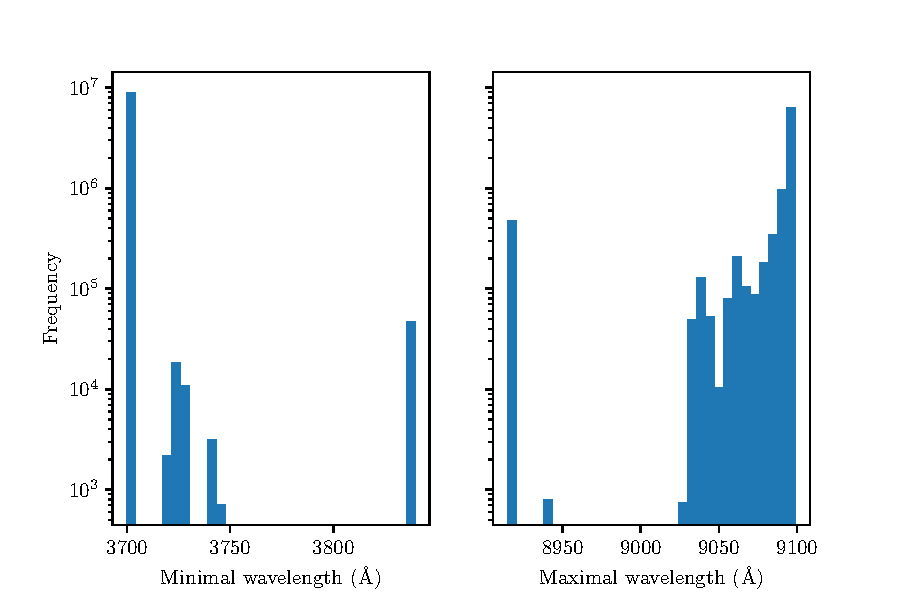
\includegraphics[width=\textwidth]{img/wavemin_wavemax_hist.pdf}
\caption[Minimal and maximal wavelength of LAMOST DR5]{
	Two plots showing histograms of minimal and maximal wavelengths
	of all LAMOST spectra.
	The maximal wavelength from all the minimal wavelengths
	is 3\,839.7244~\AA{}.
	Cutting in lower wavelength
	would mean a lost of almost 100\,000 spectra.
	The situation is very similar for maximal wavelengths
	where the minimum is 8\,914.597~\AA{}.
	Therefore, the most suitable range of wavelength is to choose
	these two wavelengths as starting and ending points.
	}
\label{wavemin_wavemax_hist}
\end{figure}

Given the selected grid of wavelength we will lose some SDSS spectra
because not all of them have all mesurement in the range.
Figure~\ref{waves_cumulative_hist} shows cumulative histogram of how many spectra we will keep for cuts in different wavelengths.
We see that major drop are behind the selected minimal and maximal wavelengths
that means we will keep most of the spectra.
Precisely, the cut will drop 34\,487 spectra from our source dataset
including 1\,949 spectra of QSO.
Therefore, the source dataset has 4\,816\,713 spectra with 627\,508 spectra of QSOs that can enter a learing of a neural network.

\begin{figure}
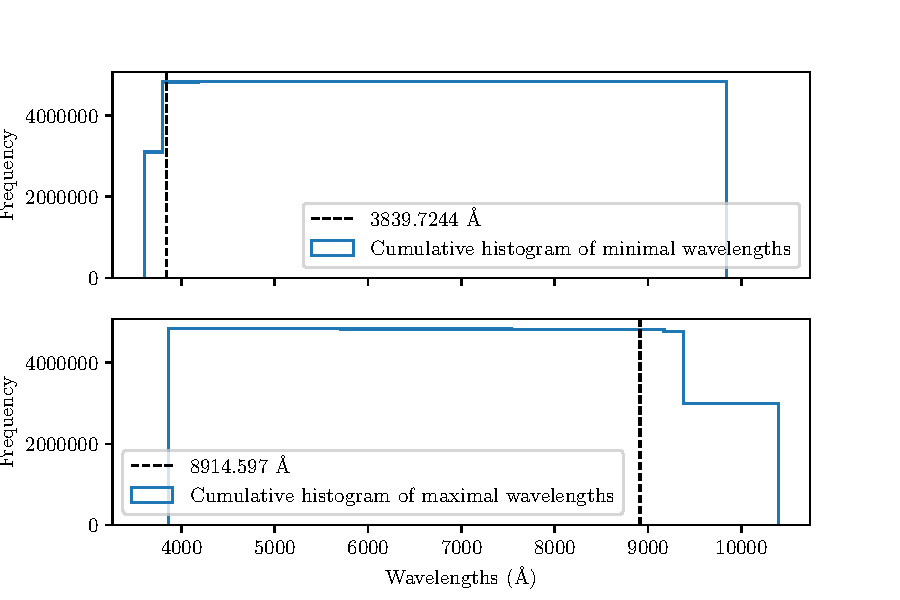
\includegraphics[width=\textwidth]{img/waves_cumulative_hist.pdf}
\caption[Losts in SDSS DR14 spectra due to wavelength range]{
	The selected wavelength range will inevitably
	cause a lost of some SDSS DR14 spectra.
	This figure show cumulative histograms of number of spectra
	and its dependence of minimal and maximal wavelengths.
	We see that both cuts are prior to big drop is count of spectra.
	}
\label{waves_cumulative_hist}
\end{figure}

The original sizes of data are unnecessary for experimenting with deep domain adataption on astronomical spectra.
We store each spectrum as a vector of 3\,659 single-precision floating-point number (4 bytes).
The storage setting gives that the SDSS source dataset has about 70.5~GB
and the LAMOST target dataset 132.1~GB.
Data of such size usually cannot fit into memory
and access to a disk significantly slows learning on a GPU.

Therefore, we have subsampled the data to the size of ImageNet~\cite{russakovsky2015}.
We believe that the size of ImageNet is more than reasonable
because ImageNet is the dataset
that enable the superiority of deep neural network in computer vision.
ImageNet has 1 million training examples, 50 thousand validation examples
and 100 thousand testing examples.
Accordingly, we randomly subsampled of source and target datasets
obtaining training sets of size 1 million
and validation sets of size 50 thousand
while the rest of the data serves as testing sets.
We summarise sizes of datasets with corresponding number of QSOs in Table~\ref{datasets_sizes}.
Table~\ref{datasets_sizes} shows a significant class imbalance in the LAMOST DR5
where QSOs are very rare (less then 0.4\%).

\begin{table}
\begin{center}
\begin{tabular}{|l|r|r|}
	\hline
	Name & QSOs & Total spectra \\
	\hline \hline
	SDSS DR14 & 629\,457 (12.98\%) & 4\,851\,200 \\ \hline
	usable SDSS DR14 & 627\,508 (13.03\%) & 4\,816\,713 \\ \hline
	SDSS training set & 130\,904 (13.09\%) & 1\,000\,000 \\ \hline
	SDSS validation set & 6\,552 (13.10\%) & 50\,000 \\ \hline
	LAMOST DR5 v3 & 31\,755 (0.35\%) & 9\,026\,365 \\ \hline
	LAMOST training set & 3\,517 (0.35\%) & 1\,000\,000 \\ \hline
	LAMOST validation set & 190 (0.38\%) & 50\,000 \\ \hline
\end{tabular}
\end{center}
\caption[Sizes of source and target datasets]{
	Summary table of sizes of source and target dataset
	together with train and validation splits.
	The validation splits serve for models comparison
	and hyperparameter optimisation.
	The second row "usable SDSS DR14" show the number of spectra
	after the cut into a unified range of wavelengths.
	The table shows the imbalance of the LAMOST target data
	that contains only tiny amount of identified QSOs.
	}
\label{datasets_sizes}
\end{table}

The last step of data preparation is min-max scaling of each spectrum into the \([-1; 1]\) range:

\begin{equation}
	\mathbf{x}_i = 2 \frac{\mathbf{x}_i - \min(\mathbf{x}_i)}{
		\max(\mathbf{x}_i) - \min(\mathbf{x}_i)} - 1,
\end{equation}

where \(\mathbf{x}_i \in \mathbb{R}^{3659}\) is a spectrum as defined in Chapter~\ref{da_chapter}
and functions \(\min(\cdot)\) and \(\max(\cdot)\) returns the smallest and the largest element of a given vectore respectively.

There are two benefits of the min-max scaling.
Firstly, the data will be in a suitable range for learning of neural networks
which will stabilise learning.
Secondly, the scaling will remove intensity properties of spectra
leaving us only with the spectrum shape which we are interesting in.

\section{Dimensionality Reduction}

In this section, we investigate the structure of joint data space of source and target datasets with three dimensionality reduction methods:
\textit{principal component analysis},
\textit{t-Distributed Stochastic Neighbor Embedding}
and \textit{Unifrom Maniforld Approximation and Projection} (UMAP).
We would like to get an idea how well are the source and target data mixed together,
if there are some separate clusters or the data are rather continuos.

To avoid visualisation overwhelmed with data points,
we sampled 2\,500 spectra from the source training set
and 2\,500 spectra from the target traininig set.
The spectra are min-max scaled not standardized
because the relation between features are meaningful
and we do not want to supress the relationship.

\textit{Principal component analysis} (PCA) is a simple linear machine learning algorithm
that is used either for visualisation or feature extraction by dimensionality reduction.
PCA learns a representation whose features are uncorrelation with each other
and selects features will the largest variation.~\cite{goodfellow2016}
We show the visualisation obtained with PCA in Figure~\ref{pca}.
The plot shows that source data tent to concenrate in the middle
while the target data are on the edges.
However, there are no regions containing only source or target data.
Moreover, in the middle extending to the right there is a kind of line component.

\begin{figure}
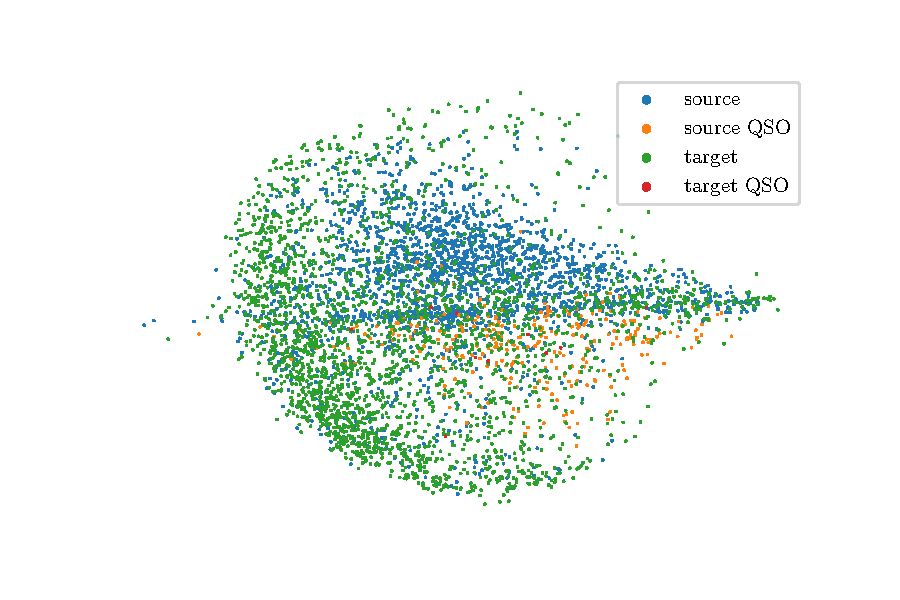
\includegraphics[width=\textwidth]{img/pca.pdf}
\caption[PCA visualisation of source and target data distributions]{
	The first two principal component of 2\,500 source
	and 2\,500 target data points.
	The projection shows that source data concentrate more in the middle
	whlie the target data seem to cluster on the edges.
	}
\label{pca}
\end{figure}

\textit{t-Distributed Stochastic Neighbor Embedding} (t-SNE)~\cite{maaten2008, wattenberg2016} is a popular method for visualisation of high-dimensional data.
The t-SNE method is non-linear, iterative
and peforms different transformation of different regions.
A tunable hyperparameter of t-SNE is \textit{perplexity}
which is a guess about the number of neighbors of a data point.
Typically, the optimal value is between 5 and 50.

We reduce dimensionality with t-SNE for perplexities from \(\{5, 10, 30, 50, 100\}\).
The best result was for the value 30
and the result is shown in Figure~\ref{tsne}.
The t-SNE embedding have similar structure to the Figure~\ref{pca} of PCA.
There are mostly source data in the center and target data around it.
However the separation between center and edges seems to be bigger.
Still ther is the line component extending to the right.

t-SNE is often used in the papers presenting a deep domain adaptation methods
to show how feature extracted from a higher layer in an adapted network
are better mix when a domain adaptation method is employed.
On the other hand, we a network is not adapted the source and target data
can be easily visually separated in a t-SNE visualisation.

\begin{figure}
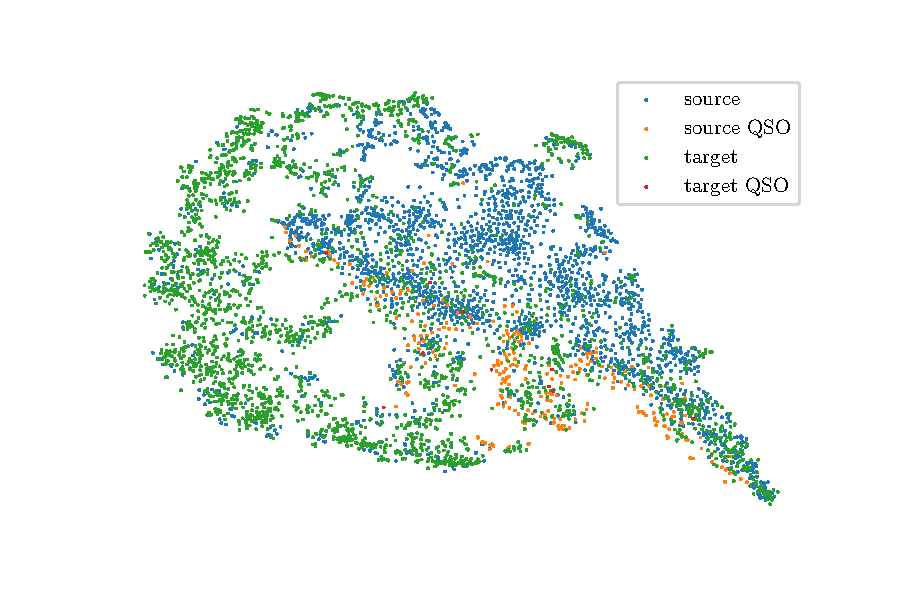
\includegraphics[width=\textwidth]{img/tsne.pdf}
\caption[t-SNE visualisation of source and target data distributions]{
	Embedding of t-SNE of the same data
	as in the reduction with PCA shows very similar result as PCA.
	However, there is more notable central sort of line component
	extending to the rigth.
	}
\label{tsne}
\end{figure}

\textit{Unifrom Manifold Approximation and Projection} (UMAP)~\cite{mcinnes2018}
is a non-linear dimensionality reduction algortihm based on manifold learning and ideas from topological data analysis.
It achieves visualisations similar to t-SNE but it is significantly faster.
Visualisation with UMAP is displayed in Figure~\ref{umap}
and have very similar structure to t-SNE embedding in Figure~\ref{tsne}.

\begin{figure}
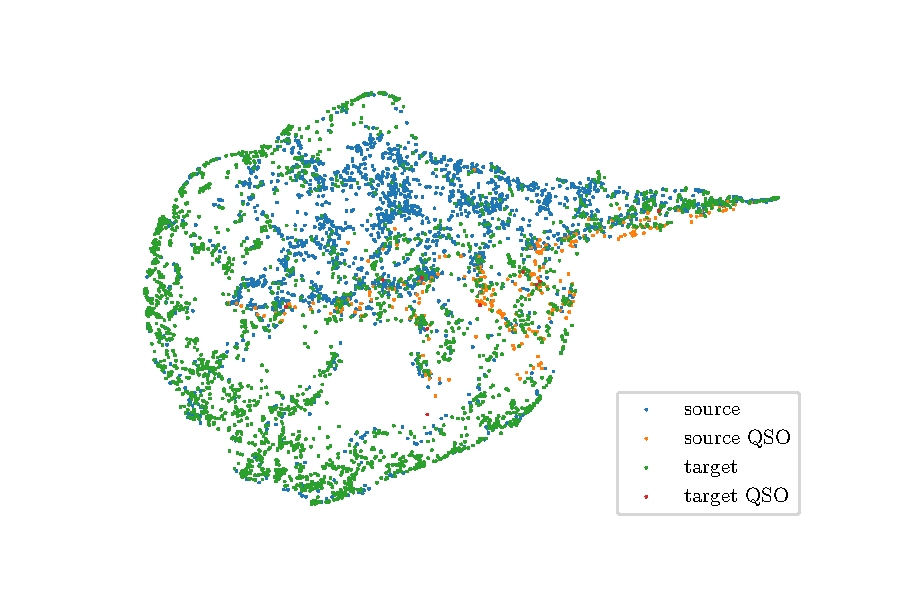
\includegraphics[width=\textwidth]{img/umap.pdf}
\caption[UMAP visualisation of source and target data distributions]{
	UMAP projection to two-dimensions confirm the previous visualisation
	with PCA and t-SNE.
	The source data tend to concentrate in the midlle
	while the target data are mostly out of center
	and there is the line component extending away from the center.
	}
\label{umap}
\end{figure}

\section{Baseline: Results without Deep Domain Adapatation}
\label{baseline}

Now, we are ready for training of neural networks
but before we will dive into deep domain adapatation
we will train a classical convulutional network
which will serve as baseline to
which we can compare results of networks augumented with deep domain adaptation.

As the baseline, we choose LeNet-5~\cite{lecun1998} convolutional neural network
which was originaly used to recognize hand written digits
of the MNIST dataset.\footnote{Available from: \url{http://yann.lecun.com/exdb/mnist/}}
We have choosen the architecture of LeNet-5
because it is the simplest model used in the DANN paper~\cite{ganin2016}.
However, the network is design for processing of two-dimensional images
while spectrum is a one-dimensional image.
Therefore, we have to substitude the two-dimensional convolutions with one-dimensional convolutions.
Moreover, we increased the kernel size and stride of pooling layer from 2 to 16
so that the output of the convolutional layer is reasonably big.
If we left the original pooling layer
the input to the first fully connected layer would be of size 43\,872.
in comparison the original input size 768 for the MNIST dataset.
The kernel size and stride of 16 will reduce the input size of our network to 672.
Figure~\ref{lenet_5} displays the final architecture
which we implemented in PyTorch~\cite{paszke2019}.

\tikzstyle{layer} = [align=center,draw=black,font=\tiny,rectangle,text centered]
\begin{figure}
\begin{center}
\subfloat[][LeNet-5]{
\begin{tikzpicture}[node distance=1.5cm]
	\node (conv1) [layer] {conv1\\5-32\\ReLU};
	\node (pool1) [layer,right of=conv1] {pool1\\16-16};
	\node (conv2) [layer,right of=pool1] {conv2\\5-48\\ReLU};
	\node (pool2) [layer,right of=conv2] {pool2\\16-16};
	\node (fc1) [layer,right of=pool2] {fc1\\100\\ReLU};
	\node (fc2) [layer,right of=fc1] {fc2\\100\\ReLU};
	\node (fc3) [layer,right of=fc2] {fc3\\1\\sigmoid};
	\draw [->] (conv1) -- (pool1);
	\draw [->] (pool1) -- (conv2);
	\draw [->] (conv2) -- (pool2);
	\draw [->] (pool2) -- (fc1);
	\draw [->] (fc1) -- (fc2);
	\draw [->] (fc2) -- (fc3);
\end{tikzpicture}
\label{lenet_5}
}\\
\subfloat[][DDC]{
\begin{tikzpicture}[node distance=1.5cm]
	\node (conv1) [layer] {conv1\\5-32\\ReLU};
	\node (pool1) [layer,right of=conv1] {pool1\\16-16};
	\node (conv2) [layer,right of=pool1] {conv2\\5-48\\ReLU};
	\node (pool2) [layer,right of=conv2] {pool2\\16-16};
	\node (fc1) [layer,right of=pool2] {fc1\\100\\ReLU};
	\node (bottleneck) [layer,right of=fc1,fill=red!50] {bottleneck\\64\\ReLU};
	\node (fc2) [layer,right of=bottleneck] {fc2\\100\\ReLU};
	\node (fc3) [layer,right of=fc2] {fc3\\1\\sigmoid};
	\draw [->] (conv1) -- (pool1);
	\draw [->] (pool1) -- (conv2);
	\draw [->] (conv2) -- (pool2);
	\draw [->] (pool2) -- (fc1);
	\draw [->] (fc1) -- (bottleneck);
	\draw [->] (bottleneck) -- (fc2);
	\draw [->] (fc2) -- (fc3);
\end{tikzpicture}
\label{ddc_architecture}
}\\
\subfloat[][DANN]{
\begin{tikzpicture}[node distance=1.5cm]
	\node (conv1) [layer] {conv1\\5-32\\ReLU};
	\node (pool1) [layer,right of=conv1] {pool1\\16-16};
	\node (conv2) [layer,right of=pool1] {conv2\\5-48\\ReLU};
	\node (pool2) [layer,right of=conv2] {pool2\\16-16};
	\node (fc1) [layer,right of=pool2,fill=blue!50] {fc1\\100\\ReLU};
	\node (fc2) [layer,right of=fc1,fill=blue!50] {fc2\\100\\ReLU};
	\node (fc3) [layer,right of=fc2,fill=blue!50] {fc3\\1\\sigmoid};
	\node (grl) [layer,below of=pool2,fill=green!50] {gradient\\reversar\\layer};
	\node (fc4) [layer,right of=grl,fill=green!50] {fc4\\100\\ReLU};
	\node (fc5) [layer,right of=fc4,fill=green!50] {fc5\\1\\sigmoid};
	\draw [->] (conv1) -- (pool1);
	\draw [->] (pool1) -- (conv2);
	\draw [->] (conv2) -- (pool2);
	\draw [->] (pool2) -- (fc1);
	\draw [->] (fc1) -- (fc2);
	\draw [->] (fc2) -- (fc3);
	\draw [->] (pool2) -- (grl);
	\draw [->] (grl) -- (fc4);
	\draw [->] (fc4) -- (fc5);
\end{tikzpicture}
\label{dann_architecture}
}\\
\subfloat[][DRCN]{
\begin{tikzpicture}[node distance=1.5cm]
	% encoder
	\node (conv1) [layer] {conv1\\5-32\\ReLU};
	\node (pool1) [layer,right of=conv1] {pool1\\16-16};
	\node (conv2) [layer,right of=pool1] {conv2\\5-48\\ReLU};
	% feature labelling
	\node (pool2) [layer,right of=conv2,fill=blue!50] {pool2\\16-16};
	\node (fc1) [layer,right of=pool2,fill=blue!50] {fc1\\100\\ReLU};
	\node (fc2) [layer,right of=fc1,fill=blue!50] {fc2\\100\\ReLU};
	\node (fc3) [layer,right of=fc2,fill=blue!50] {fc3\\1\\sigmoid};
	% decoder
	\node (conv3) [layer,below of=conv2,fill=green!50] {conv3\\5-48\\ReLU};
	\node (upsample1) [layer,left of=conv3,fill=green!50] {upsample1\\3659};
	\node (conv4) [layer,left of=upsample1,fill=green!50] {conv4\\5-32\\None};
	% connections
	\draw [->] (conv1) -- (pool1);
	\draw [->] (pool1) -- (conv2);
	\draw [->] (conv2) -- (pool2);
	\draw [->] (pool2) -- (fc1);
	\draw [->] (fc1) -- (fc2);
	\draw [->] (fc2) -- (fc3);
	\draw [->] (conv2) -- (conv3);
	\draw [->] (conv3) -- (upsample1);
	\draw [->] (upsample1) -- (conv4);
\end{tikzpicture}
\label{drcn_architecture}
}
\end{center}
\caption[Architectures of deep domain adaptation model from experiments]{
	Diagrams of all architectures used in our experiments.
	}
\end{figure}

Furthermore, Donahue et al. showed in the DeCAF (\textit{Deep Convolutional Activation Feature}) paper~\cite{donahue2014}
that features extracted from deep CNN can be repurposed to novel tasks
if the network were trained on a large fixed set in fully supervised fashion.
Meaning that it can be used for domain adaptation on its own.
Therefore, we can expected that our CNN trained on the large SDSS
will be able to find features beneficial for domain adaptation.
Still the DeCAF paper showed that
deep CNN cannnot remove domain bias completelly.
Therefore, there is a space for improvement with deep domain adaptation
and DDC, Deep CORAL and DANN build in experiment on result of DeCAF
because they use AlexNet~\cite{krizhevsky2012} pre-trained on ImageNet dataset.

We trained our adapted LeNet-5 on batches of size 64 for 20 epochs
with the Adam optimiser~\cite{kingma2014} in its default setting
and used the \textit{binary cross entropy loss} defined as:

\begin{equation}
	\mathit{BCE}(\theta) = -\frac{1}{M} \sum_i^M [y_i \log \hat{y}_i + (1 - y_i) \log(1 - \hat{y}_i)],
\end{equation}

where \(\theta\) are all parameters of a model,
\(M\) is the batch size,
\(y_i \in \{0, 1\}\) is the true label
and \(\hat{y}_i \in [0, 1]\) are the model predictions of the \(i\)-th example in the batch.
Furthermore, we intialised the weights and biases in accordance with Xavier initialisation~\cite{glorot2010}.
That is weights of our neural network are sampled from uniform distribution \(\mathcal{U}\):

\begin{equation}
	\mathcal{U}\left(
	-\frac{\sqrt{6}}{\sqrt{\mathit{in} + \mathit{out}}},
	\frac{\sqrt{6}}{\sqrt{\mathit{in} + \mathit{out}}}
	\right),
\end{equation}

where \(\mathit{in}\) is the number of input units of a layer
and \(\mathit{out}\) is the number of output units
and biases are set to zero.

% TODO training progress

\begin{figure}
	\subfloat[][Losses]{
		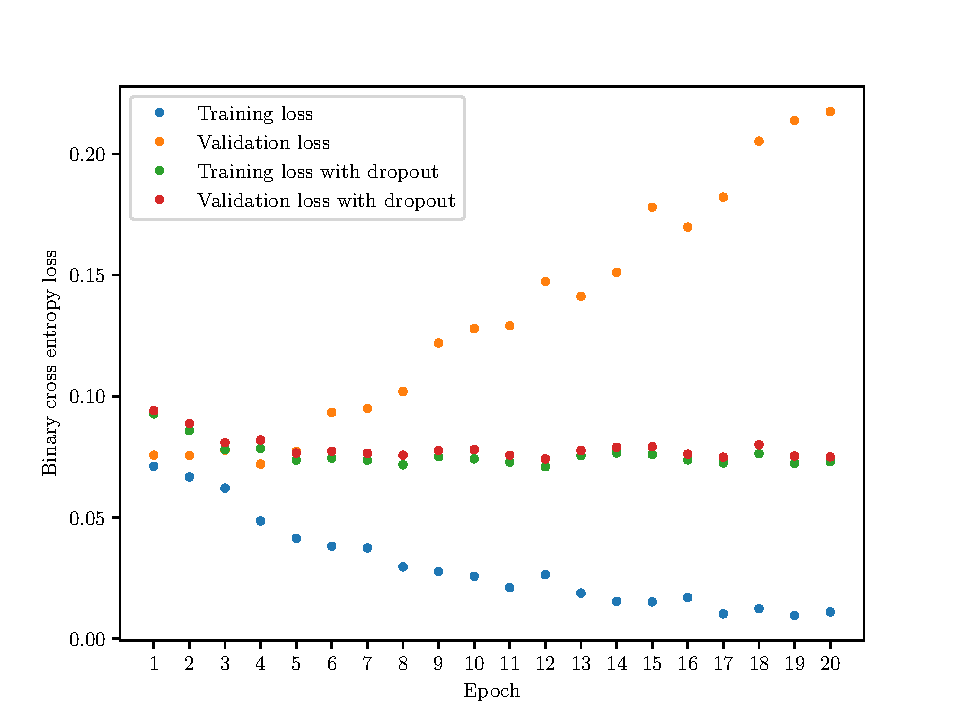
\includegraphics[width=.5\textwidth]{img/lenet_losses.pdf}
	}
	\subfloat[][\(F_1\) score]{
		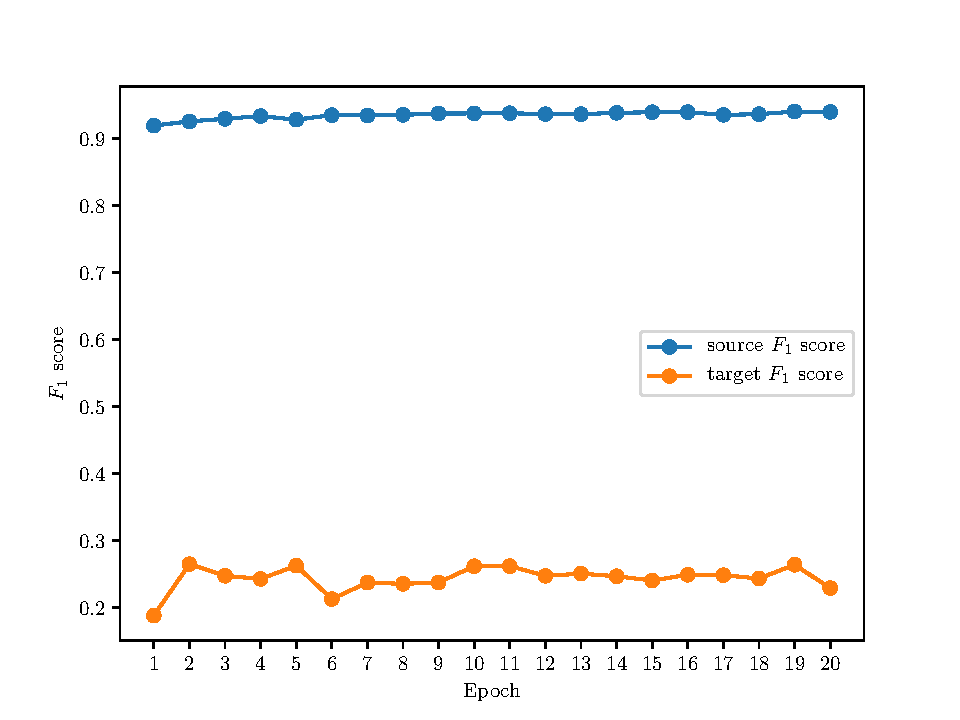
\includegraphics[width=.5\textwidth]{img/lenet_f1.pdf}
	}
	\caption{Training of LeNet-5}
	\label{lenet_losses}
\end{figure}

\textit{Recall} \(r\), \textit{precision} \(p\)
and \textit{\(F_1\) score} is the harmonic mean between \textit{precision} and \textit{recall}:

\begin{align}
	r &= \frac{\mathit{TP}}{\mathit{TP} + \mathit{FN}}, \\
	p &= \frac{\mathit{TP}}{\mathit{TP} + \mathit{FP}}, \\
	F_1 &= \frac{2}{r^{-1} + p^{-1}} = 2 \frac{r p}{r + p},
\end{align}

where \(r\) is recall, \(p\) is precision,
\(\mathit{TP}\) is the number of correctly classified QSOs,
\(\mathit{FN}\) is the number of QSOs incorrectly classified as non-QSOs
and \(\mathit{FP}\) is the number of non-QSOs classified as QSOs.
When precision and recall are perfect
\(F_1\) score reaches its best value one and at worst can be zero.

Validation \(F_1\) score of source is 0.9397 and target 0.2294
(target precision is is 13.48\% and target recall 76.84\%).
That is a very poor result for the target data.
Therefore, we see that there probably is a huge domain discrepancy.

\begin{table}
\begin{center}
\subfloat[][Source confusion matrix]{
	\begin{tabular}{|l|r|r|}
		\hline
		Predicted class & \multicolumn{2}{c|}{Actual class} \\
		\hline \hline
		& QSO & non-QSO \\ \hline
		QSO & 6\,278 & 532 \\ \hline
		non-QSO & 274 & 42\,916 \\ \hline
	\end{tabular}
}
\subfloat[][Target confusion matrix]{
	\begin{tabular}{|l|r|r|}
		\hline
		Predicted class & \multicolumn{2}{c|}{Actual class} \\
		\hline \hline
		& QSO & non-QSO \\ \hline
		QSO & 146 & 937 \\ \hline
		non-QSO & 44 & 48\,873 \\ \hline
	\end{tabular}
}
\end{center}
\end{table}

\section{Experiments with Deep Domain Adapation}

We set the baseline result with classical CNN.
Now, we apply four deep domain adaptation method to the same data
to show if astronomical spectroscopy can benefit from domain adapation
based on neural networks.

We start with two discrepancy-based approach which are DDC and Deep.
Then, we continue will DANN
which is an adversarial-based domain adaptation method
and we with reconstruction based DRCN.
We conclude with evaluation and comparison of results.

\subsection{DDC: Deep Domain Confusion}

Firts deep domain adaptation method is \textit{Deep Domain Confusion} (DDC).
DDC reduces the domain discrepancy (maximises domain confusion)
by extending classification loss of a neural network with the MMD loss
(see Equation~\ref{ddc_loss}).
The MMD loss is enforced on \textit{adaptation layer}
that serves information bottleneck for domain confusion.
More details on DDC are in Subsection~\ref{discrepancy_da}.

To select the size and placement of the adaptation layer,
we followed the same procedure as in the DDC paper~\cite{tzeng2014}.
Firstly, we took the LeNet-5 trained in previous Section~\ref{baseline}
and extracted features from the first and second fully-connected layer
(the last fully-connected layer has a trivial width)
for all validation examples.
Then, we computed MMD between the source and target data at each layer with the extracted features.
The intuition is to place the adaptation layer after a layer with smallest MMD
because low MMD means more domain invariant features.
We measured that the MMD at the first fully-connected layer is 50.70
while MMD at the second fully-connected layer is 53.33.
Therefore, we will place the adaptation layer after the first fully-connected layer.
Secondly, we have to optimise the width of the adapataion layer.
Therefore, we trained the LeNet with the adapation layer of sizes
from \(\{4, 8, 16, 32, 64\}\) excluding the low width of 2
and not exceeding the output size of previous layer.
The stepping is power of two as in the original paper.
Figure~\ref{adaptation_layer} plots the resulting MMD values for different setting
and shows that the width 64 is the best.

The final architecture of our DDC network is in Figure~\ref{ddc_architecture}.
It is the baseline CNN with the adapatation layer of width 64
after the first fully-connected layer.

\begin{figure}
	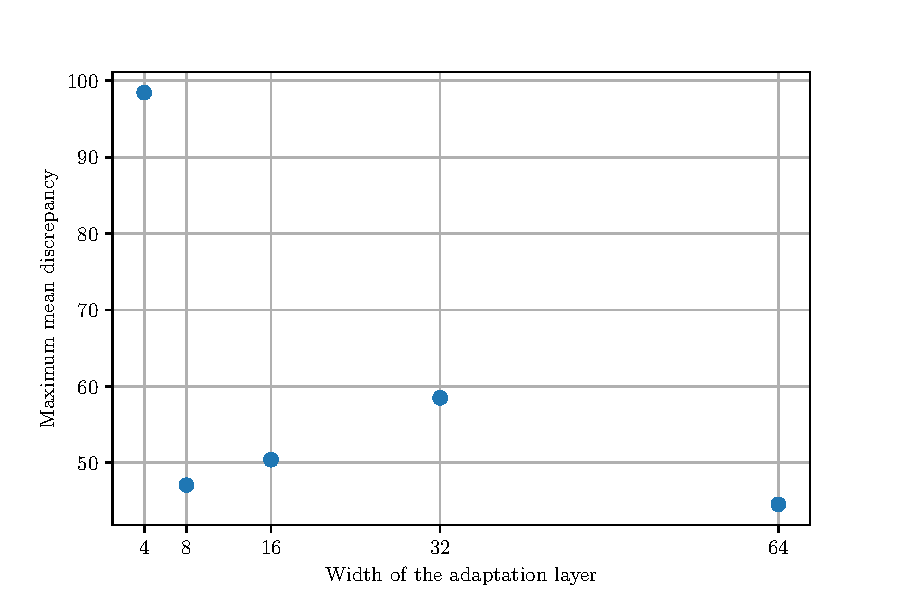
\includegraphics[width=\textwidth]{img/adaptation_layer_width.pdf}
	\caption{Width of the adapation layer}
	\label{adaptation_layer}
\end{figure}

Furthermore, we set the trade-off parameter \(\lambda\)
between the binary cross entropy loss
and the MMD loss to 0.25 as in the DDC experiments
and trained the network in the same way as described in previous section~\ref{baseline}
(Xavier initialisation, Adam optimizer, batch size 64 and 20 epochs).

Figure~\ref{ddc_training} displays training progress of DDC
which is correctly learning to classify.
Moreover, we see that MMD is also minimalised in the bottom plot of Figure~\ref{ddc_mmds}
while if we train the network without enforcing MMD loss (\(\lambda = 0\))
then the MMD is growing as in the top plot of Figure~\ref{ddc_mmds}.

\begin{figure}
\subfloat[][Losses]{
	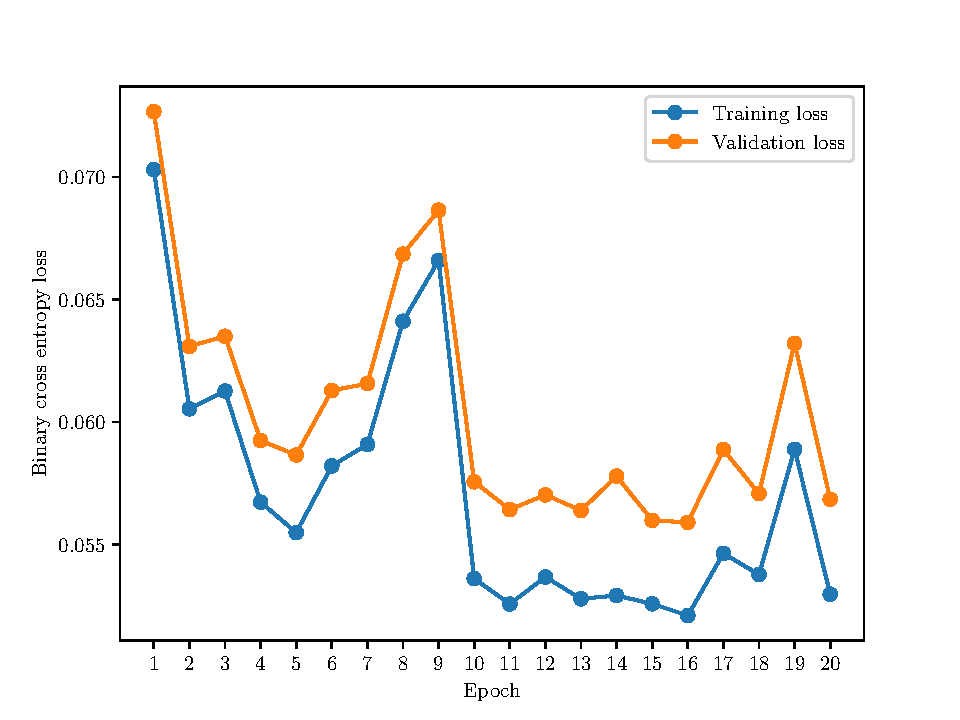
\includegraphics[width=.5\textwidth]{img/ddc_losses.pdf}
}
\subfloat[][Maximum mean discrepancy]{
	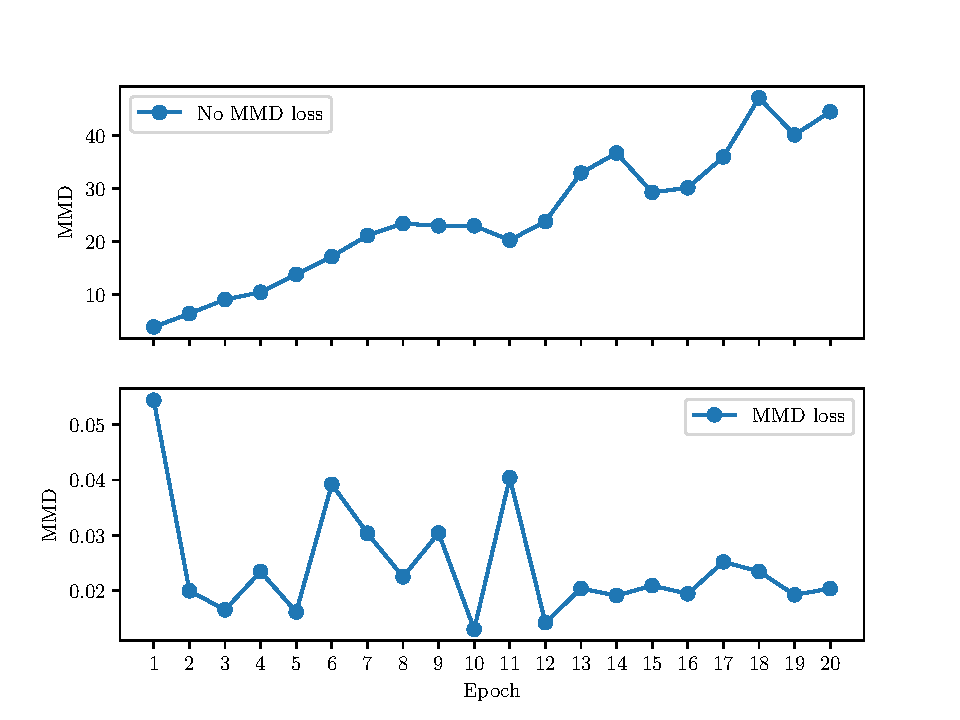
\includegraphics[width=.5\textwidth]{img/ddc_mmds.pdf}
	\label{ddc_mmds}
}
\caption{Training of DDC}
\label{ddc_training}
\end{figure}

Although, training run as expected
DDC achived poor result in comparison to baseline.
The \(F_1\) score on source data is 0.9354 and on target 0.2005
that is lower than the baseline in both cases.
Precision on target is 11.51\% and
the only imporovement is recall of value 77.89\%
but that is probably caused by the decrease in precision.
Table~\ref{ddc_confusion} shows a confusion matrix of the result.

\begin{table}
	\begin{center}
	\begin{tabular}{|l|r|r|}
		\hline
		Predicted class & \multicolumn{2}{c|}{Actual class} \\
		\hline \hline
		& QSO & non-QSO \\ \hline
		QSO & 148 & 1\,138 \\ \hline
		non-QSO & 42 & 48\,672 \\ \hline
	\end{tabular}
	\end{center}
	\caption{Target confusion matrix}
	\label{ddc_confusion}
\end{table}

\subsection{Deep CORAL: Deep Correlation Alignment}

\textit{Deep Correlation Alignment} (Deep CORAL) is very similar to DDC.
While DDC aligns means of source and target distributions with MMD loss
Deep CORAL aligns correlations with CORAL loss
(see Equations~\ref{coral_loss} and \ref{deep_coral_loss}).
Moreover, Deep CORAL applies the CORAL loss straight to a layer in a network
not creating an adaptation layer.
We implemented Deep CORAL with inspiration from original
code\footnote{Available from: \url{https://github.com/visionlearninggroup/CORAL}}
and follow all the step described in corresponding paper~\cite{sun2016}.

Originally, the architecture underlying Deep CORAL is AlexNet~\cite{krizhevsky2012}.
There the CORAL loss was put on the last layer that has ten output units.
However, our neural network has to have one output unit
so applying CORAL loss does not make sense.
Therefore, we applied the CORAL loss to the second fully-connected layer
of our LeNet-5 architecture in Figure~\ref{lenet_5}.
Then, we optimised the trade-off between classification and CORAL loss
\(\lambda\) from \(\{0.5, 0.1, 0.05, 0.01, 0.005, 0.001, 0.0005, 0.0001\}\).
The best is \(\lambda = 0.0005\) which makes the calssification loss
and the CORAL loss of similar magnitude as suggested by the paper
(see Figure~\ref{deep_coral_losses}).
Furthermore, we used the same batch size of value 128
as in original experiments of Deep CORAL.
The architecture is intialised in the same way as baseline
and optimised with Adam for 20 epochs.

Firstly, we trained our Deep CORAL with \(\lambda = 0\) to see
how the correlation alignment grows.
Figure~\ref{deep_coral_coral} shows the same behavior of correlation alignment
without enforcing the minimisation of correlation loss as in the original paper.
Then, we carried out experiment with the best \(\lambda = 0.0005\)
and obtained the training progress in Figure~\ref{deep_coral_losses}.
However, the result are unsatisfactory as in the case of DDC.

\begin{figure}
	\subfloat[][Training of Deep CORAL]{
		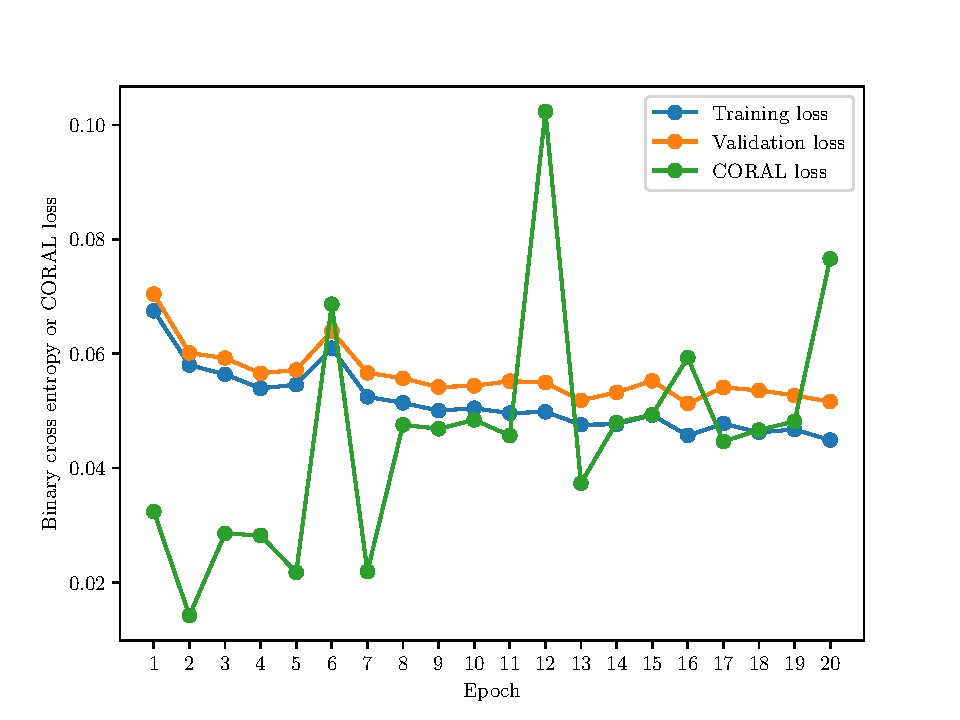
\includegraphics[width=.5\textwidth]{img/deep-coral_losses.pdf}
		\label{deep_coral_losses}
	}
	\subfloat[][CORAL with using CORAL loss]{
		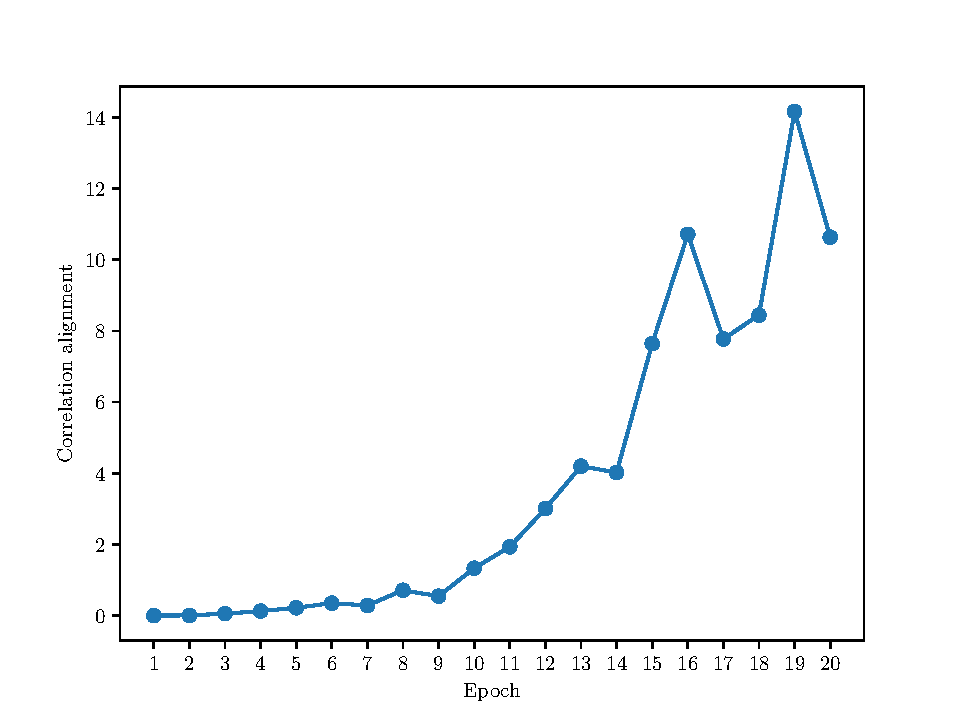
\includegraphics[width=.5\textwidth]{img/deep-coral_coral.pdf}
		\label{deep_coral_coral}
	}
	\caption{Losses of Deep CORAL}
\end{figure}

Source data \(F_1\) score is of value 0.9396
that is almost the same as baseline
and there is also a small but insignificant imporovement in the target \(F_1\) score
which is of value 0.2509.
Target precision is 14.97\% and target recall is 77.37\%.
These values are gains but their are too small
and the model with such small precision is useless for identification of QSOs.

\begin{table}
\begin{center}
\begin{tabular}{|l|r|r|}
	\hline
	Predicted class & \multicolumn{2}{c|}{Actual class} \\
	\hline \hline
	& QSO & non-QSO \\ \hline
	QSO & 147 & 835 \\ \hline
	non-QSO & 43 & 48\,975 \\ \hline
\end{tabular}
\end{center}
\caption{Target confusion matrix of Deep CORAL}
\end{table}

\subsection{DANN: Domain-Adversarial Neural Network}

\textit{Domain-Adversarial Neural Network} (DANN) is an adversarial-based domain adaptation method.
Our DANN architecture is depicted in Figure~\ref{dann_architecture}.
It consist of a feature extractor, a predictor and a domain classifier
that acts adversarially agains the feature extractor
enforcing domain invariant representation.
Further details are in Subsection~\ref{adversarial_da}.

We code and schedule hyperparameters of DANN accoring to original
implementation\footnote{Available from: \url{http://sites.skoltech.ru/compvision/projects/grl/}}
and two papers where DANN was published~\cite{ganin2015, ganin2016}.
The learning rate schedule for SGD with momentum:

\begin{equation}
	\mu_p = \frac{\mu_0}{(1 + \alpha p)^\beta},
\end{equation}

where \(p\) is the training progress linearly changign from 0 to 1 in every iteration,
initial learning rate \(\mu_0 = 0.01\), \(\alpha = 10\) and \(\beta = 0.75\).

The domain adaptation parameter \(\lambda\) from Equation~\ref{dann_loss}
start at 0 and grows to 1 with schedule:

\begin{equation}
	\lambda_p = \frac{2}{1 + e^{-\gamma p}} - 1,
\end{equation}

where \(p\) is again the training progress
and \(\gamma\) that was set to 10 in the original paper.

\begin{figure}
	\subfloat[][Training losses of DANN]{
		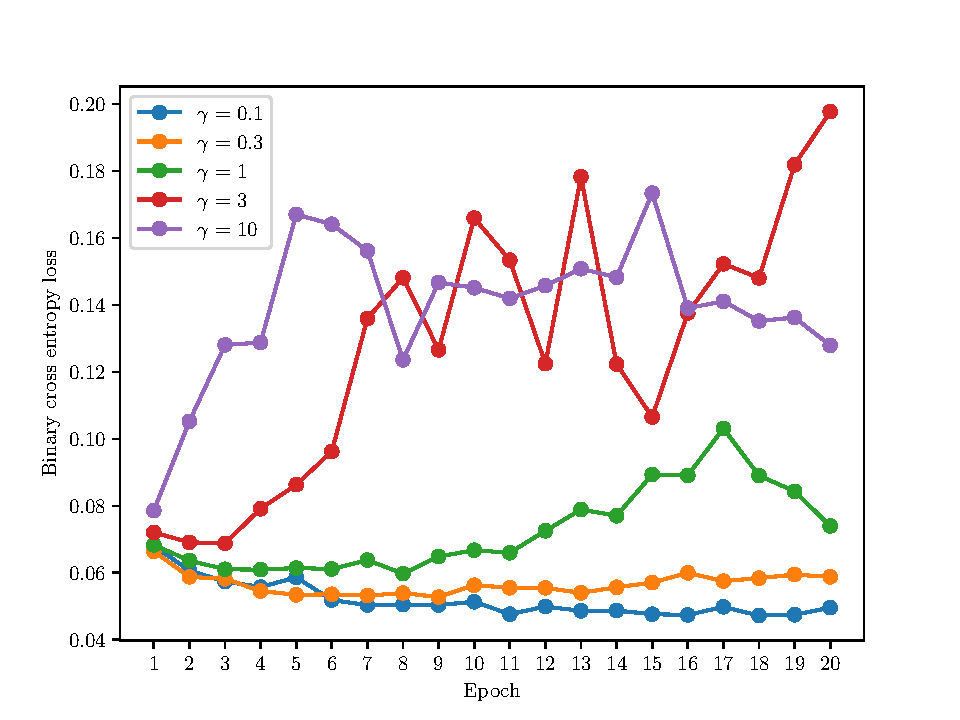
\includegraphics[width=.5\textwidth]{img/dann_losses.pdf}
	}
	\subfloat[][\(F_1\) score for different \(\gamma\)]{
		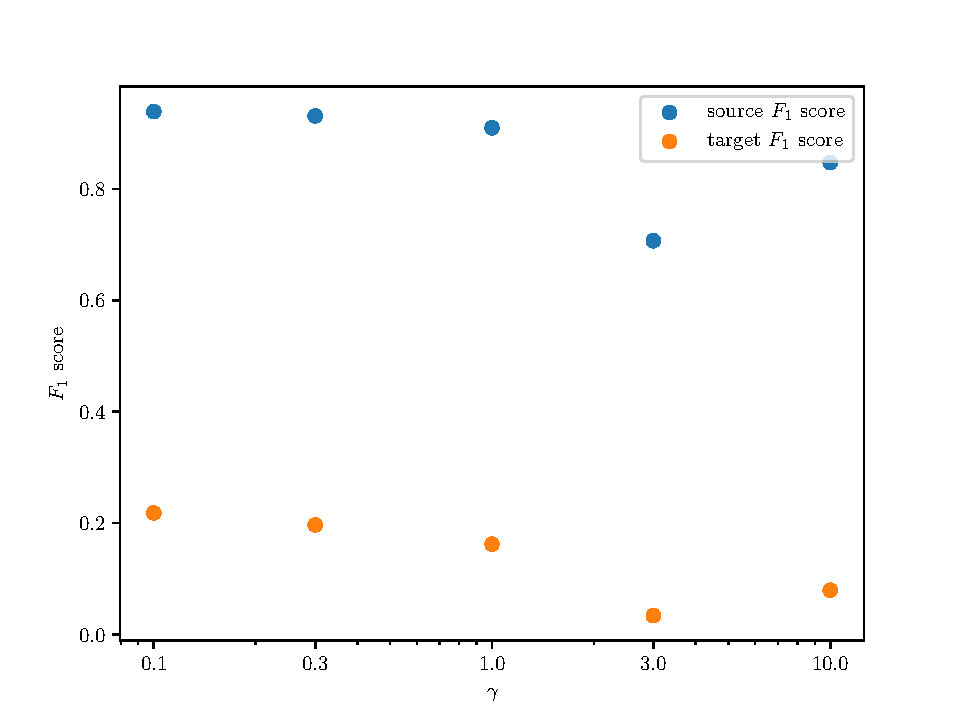
\includegraphics[width=.5\textwidth]{img/dann_f1.pdf}
	}
	\caption{Training of DANN}
	\label{dann_training}
\end{figure}

Note that binary cross entropy loss is used for both the classification and domain loss.
The optimiser is SGD with the learning rate schedule and momentum 0.9,
the network is initialised as our baseline model
and the batch size is 128 where first half are source domain data
and the second half are the target domain data.

Although following the original impelementation as closely as possible
and doing hyperparameter optimisation of \(\gamma \in \{0.1, 0.3, 1, 3, 10\}\)
we were not able to get reasonable results with DANN.
We infer from Figure~\ref{dann_training} that
if gamma is high the training will diverge.
On the other hand, if gamma is low \(F_1\) score regress.

\subsection{DRCN: Deep Reconstruction-Classification Network}

The last deep domain adaptation model is
\textit{Deep Reconstruction-Classification Network} (DRCN)
which uses reconstruction of target data as auxiliary task.
Intuition is that the auxiliary task
will enfore the network to capture also the structure of target data space.
More detail are provided in~Subsection~\ref{reconstruction_da}.

We followed the original implementation\footnote{Available from: \url{https://github.com/ghif/drcn}} of DRCN~\cite{ghifary2016}.
There is one big difference between the original paper and the official paper
that is the order of training loops.
The paper states that the network in an epoch
should firstly be trained for classification task
and then for reconstruction task.
The implementation work the other way around.

We followed the working implementation and train for reconstruction first.
Accordingly, we used Adam optimiser with batch size 128 for 20 epochs
and Xavier initialisation.
The trade-off parameter \(\lambda\) was set to 0.5.
Figure~\ref{drcn_training} shows the training progress
and Figure~\ref{reconstruction} show that the network is able to learn
good representation that can supress noise
while maitaining important spectral lines.

\begin{figure}
\subfloat[][Validation reconstruction loss of DRCN]{
	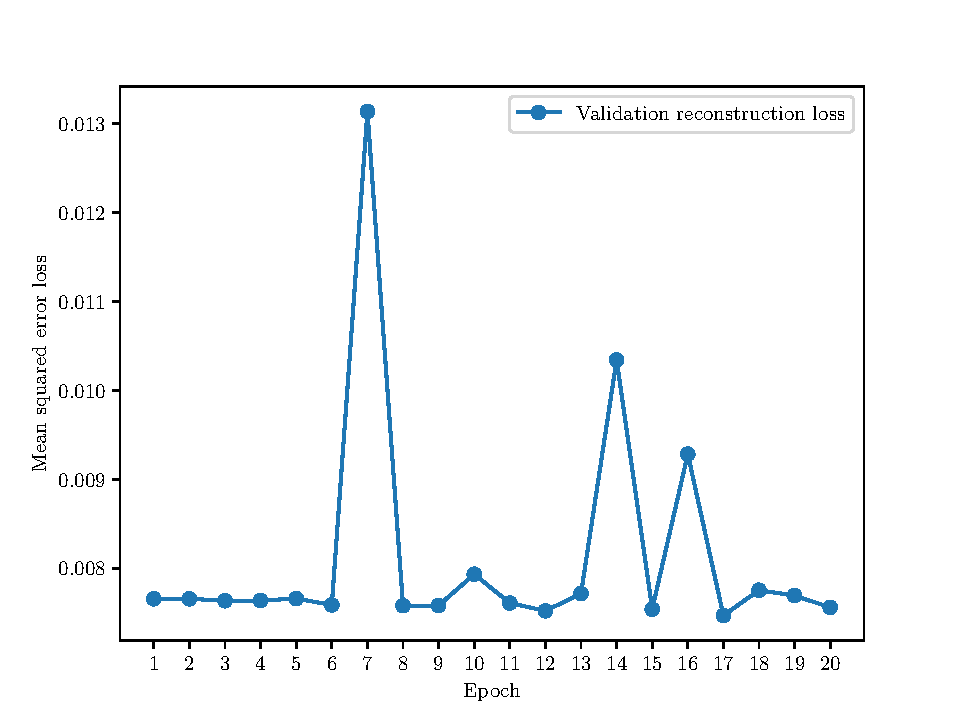
\includegraphics[width=.5\textwidth]{img/drcn_rec-loss.pdf}
}
\subfloat[][\(F_1\) score of DRCN and our LeNet-5]{
	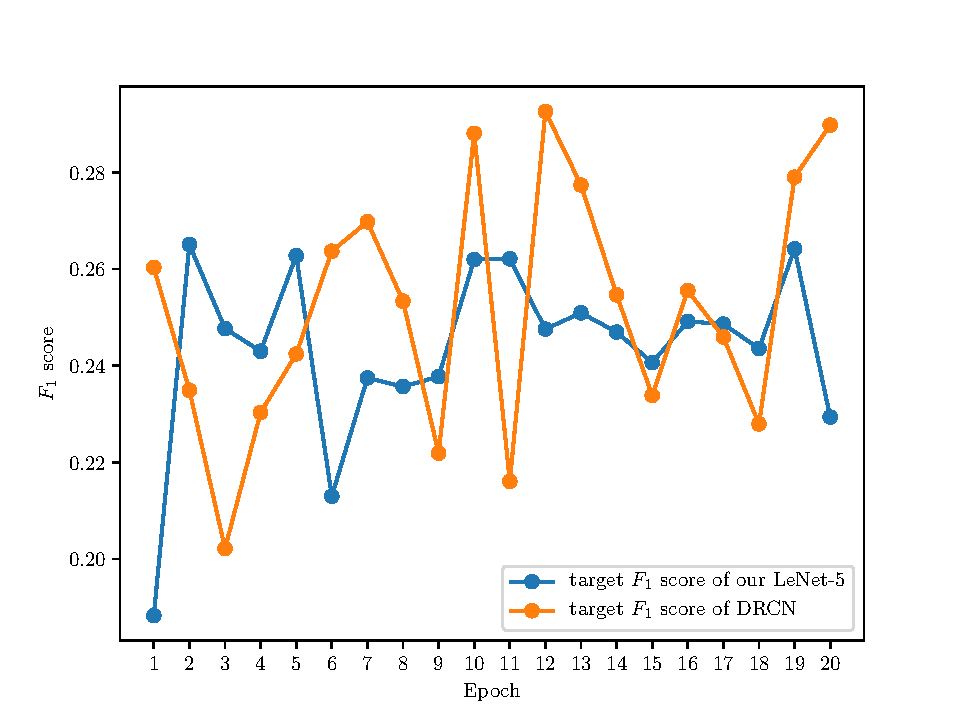
\includegraphics[width=.5\textwidth]{img/drcn_f1.pdf}
	\label{drcn_f1}
}
\caption{Training of DRCN}
\label{drcn_training}
\end{figure}

\begin{figure}
	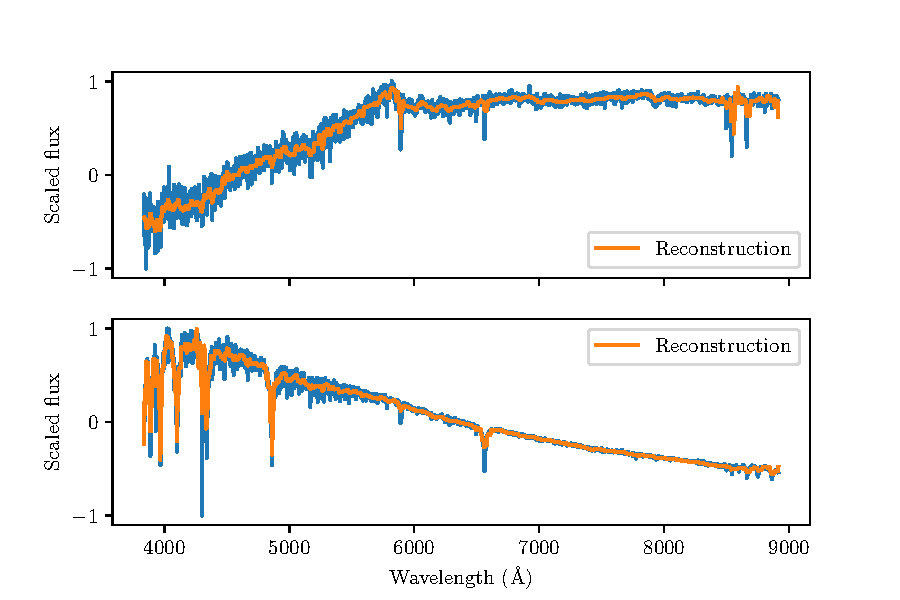
\includegraphics[width=\textwidth]{img/reconstructed_spectra.pdf}
	\caption{Spectra reconstructed with DRCN}
	\label{reconstruction}
\end{figure}

However, achiving poor results with previous methods
we did not suppose to get good result now.
Source \(F_1\) score is 0.9393 and target \(F_1\) score 0.2898
which is better than baseline
but the development of the \(F_1\) score in Figure~\ref{drcn_f1} suggest no significance.
Target precision is 17.97\% whcich si the best so far
but target recall 74.74\% is the worst.

\begin{table}
\begin{center}
\begin{tabular}{|l|r|r|}
	\hline
	Predicted class & \multicolumn{2}{c|}{Actual class} \\
	\hline \hline
	& QSO & non-QSO \\ \hline
	QSO & 142 & 648 \\ \hline
	non-QSO & 48 & 49\,162 \\ \hline
\end{tabular}
\end{center}
\caption{Target confusion matrix of DRCN}
\end{table}

\section{Evaluation of Experiments}

\begin{table}
\begin{center}
\begin{tabular}{|l|r|r|r|r|}
	\hline
	Method & Source \(F_1\) & Target \(F_1\) & Precision (\%) & Recall (\%) \\
	\hline \hline
	Baseline & 0.9397 & 0.2294 & 13.48 & 76.84 \\ \hline
	DDC & 0.9354 & 0.2005 & 11.51 & 77.89 \\ \hline
	Deep CORAL & 0.9396 & 0.2509 & 14.97 & 77.37 \\ \hline
	DRCN & 0.9393 & 0.2898 & 17.97 & 74.74 \\ \hline
\end{tabular}
\end{center}
\caption{Summary table}
\end{table}

Prepare visualisation of results.

\begin{figure}
\subfloat[][]{
	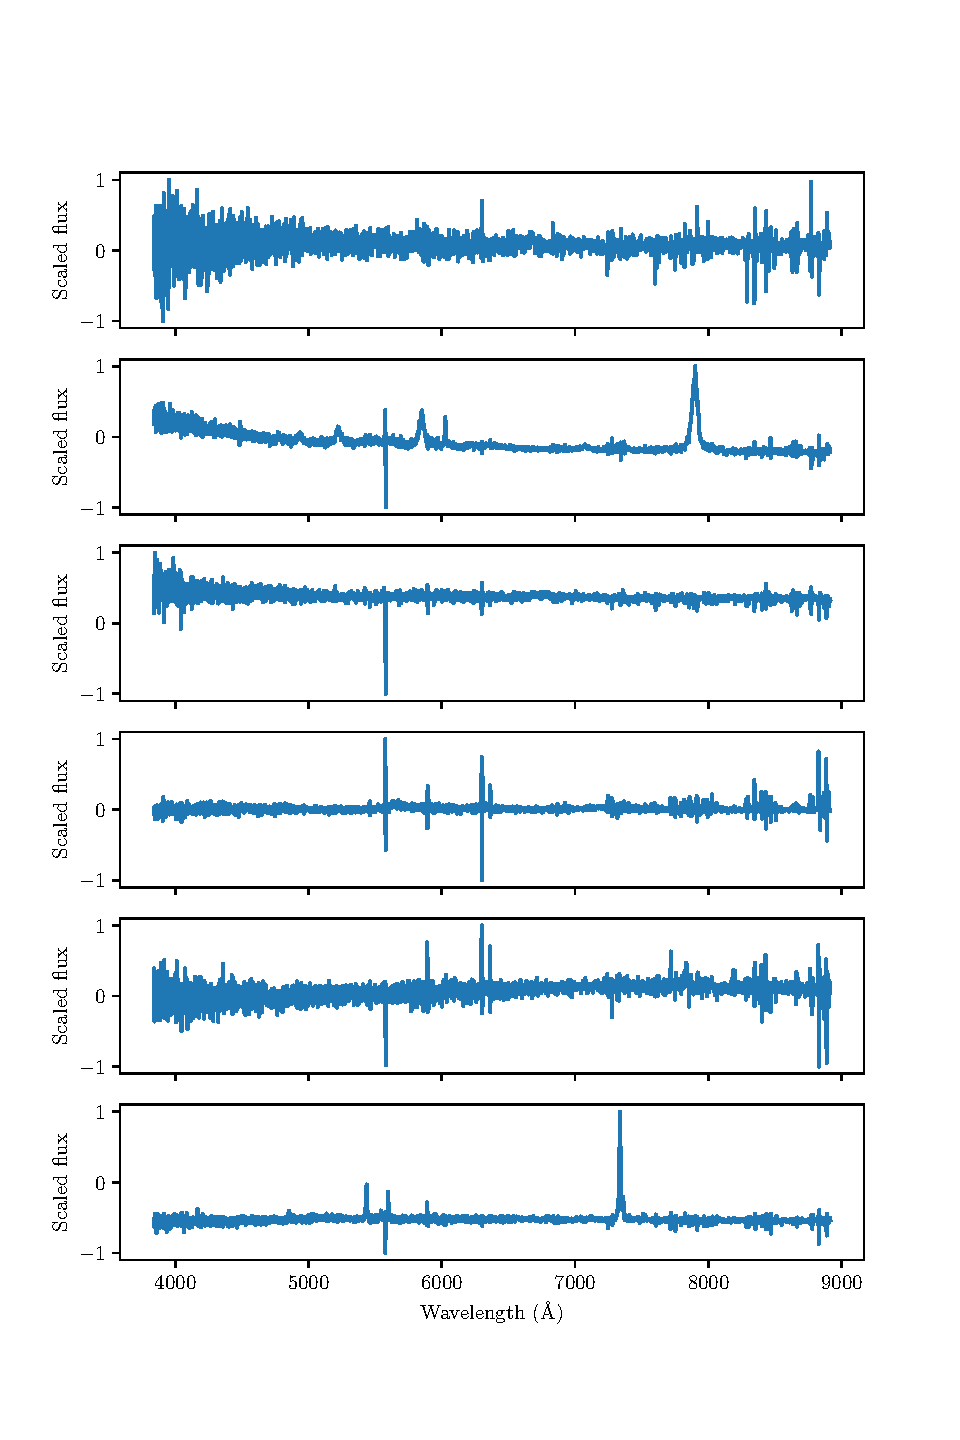
\includegraphics[width=.5\textwidth]{img/source_fn.pdf}
}
\subfloat[][]{
	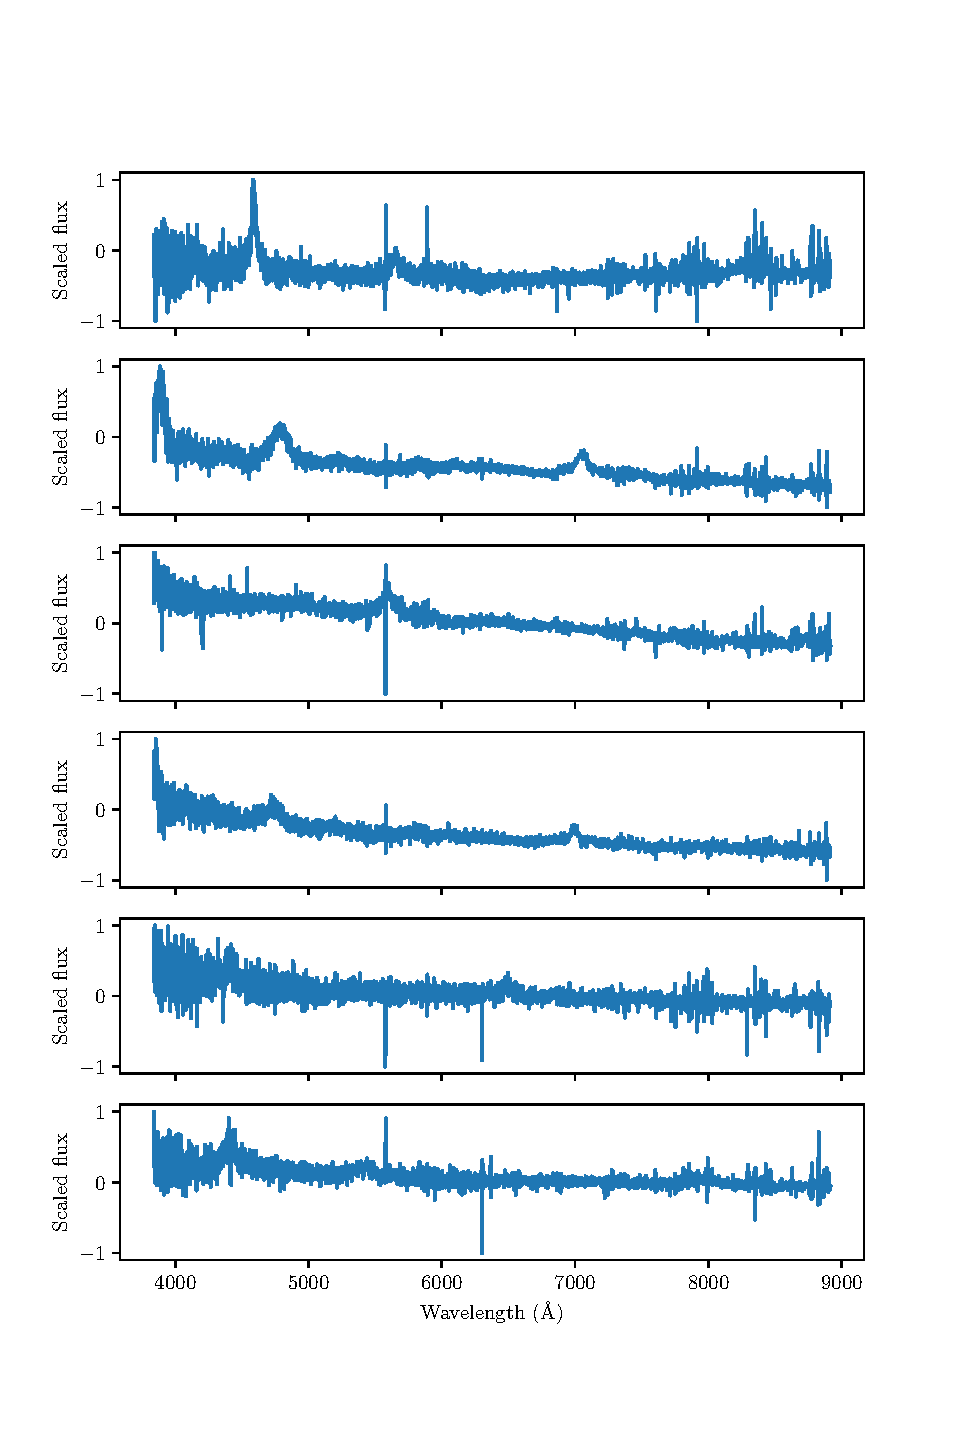
\includegraphics[width=.5\textwidth]{img/source_fp.pdf}
}
\caption{Source FN and FP}
\end{figure}

\begin{figure}
\subfloat[][]{
	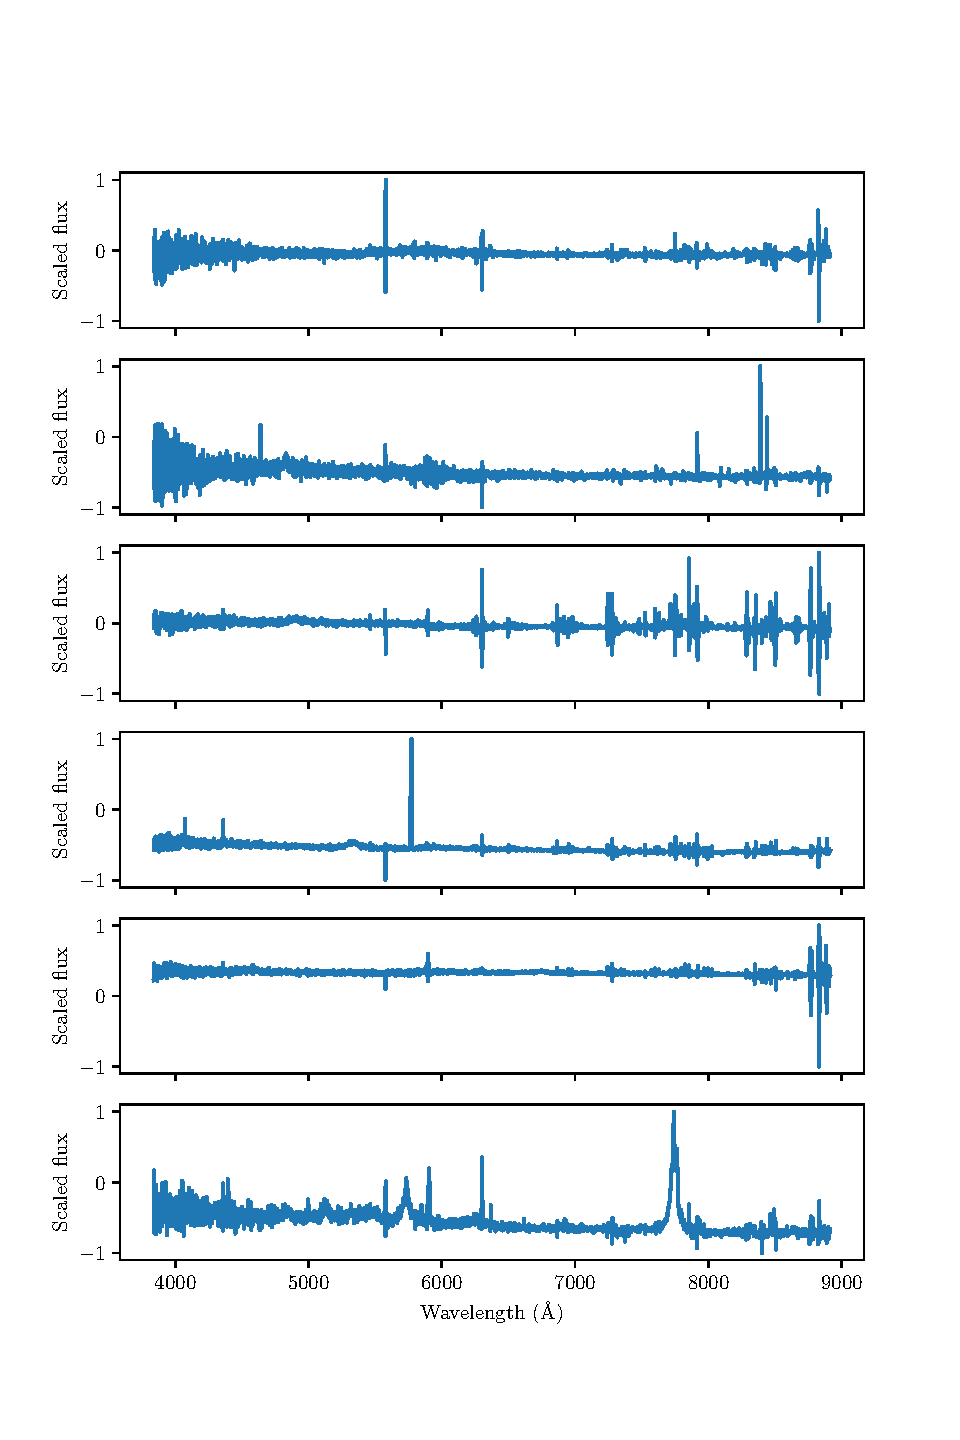
\includegraphics[width=.5\textwidth]{img/target_fn.pdf}
}
\subfloat[][]{
	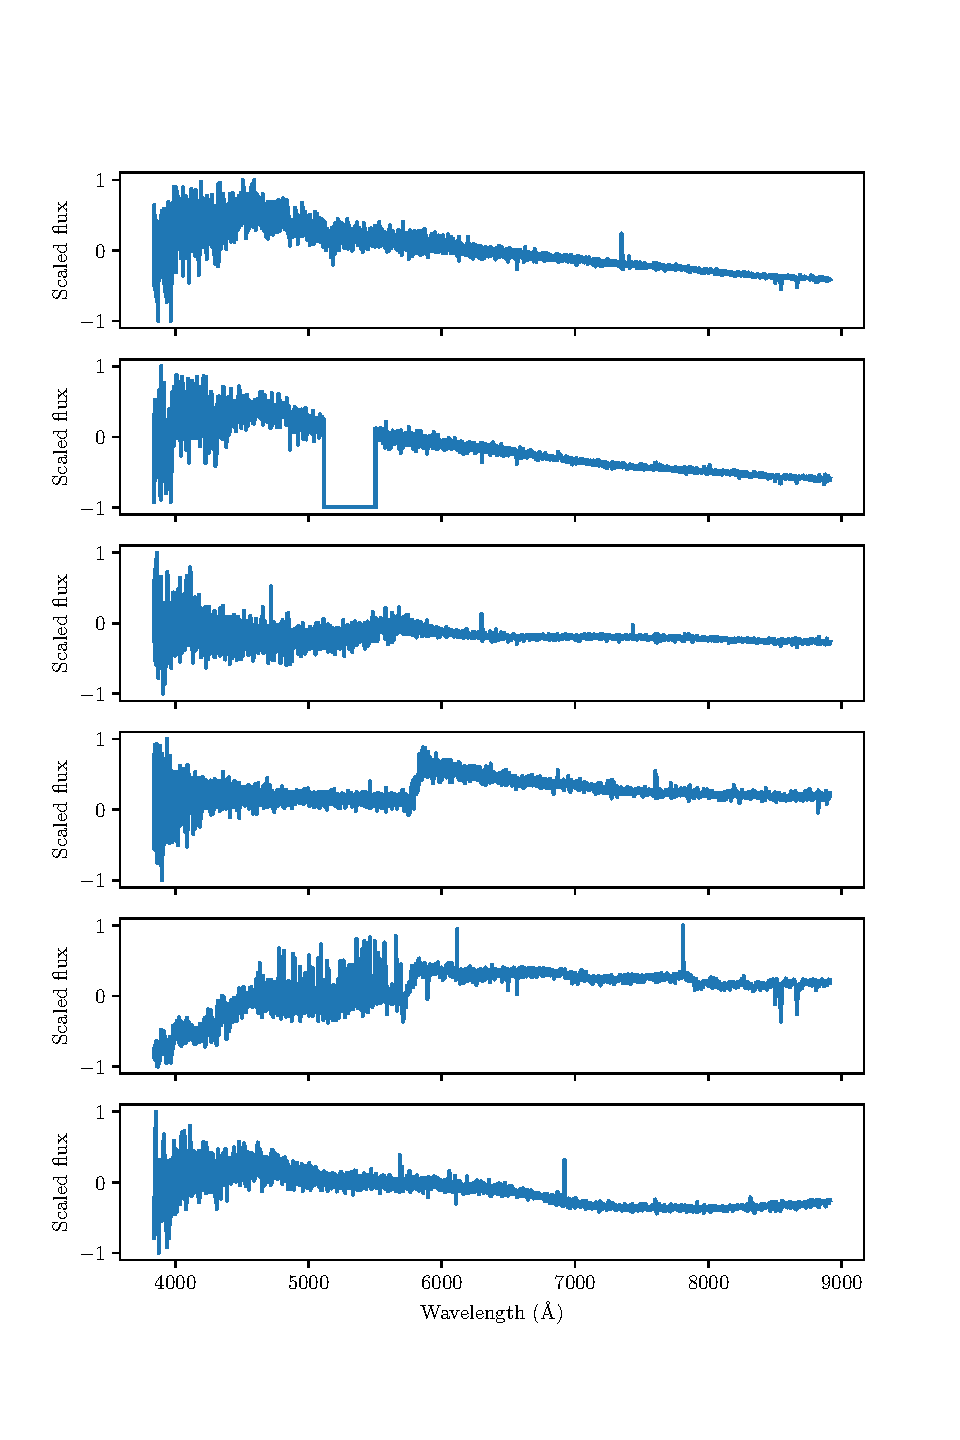
\includegraphics[width=.5\textwidth]{img/target_fp.pdf}
}
\caption{Target FN and FP}
\end{figure}
